% Generated by Sphinx.
\def\sphinxdocclass{report}
\documentclass[letterpaper,10pt,english]{sphinxmanual}
\usepackage[utf8]{inputenc}
\DeclareUnicodeCharacter{00A0}{\nobreakspace}
\usepackage{cmap}
\usepackage[T1]{fontenc}
\usepackage{babel}
\usepackage{times}
\usepackage[Bjarne]{fncychap}
\usepackage{longtable}
\usepackage{sphinx}
\usepackage{multirow}


\title{enuActor Documentation}
\date{May 20, 2014}
\release{}
\author{Author}
\newcommand{\sphinxlogo}{}
\renewcommand{\releasename}{Release}
\makeindex

\makeatletter
\def\PYG@reset{\let\PYG@it=\relax \let\PYG@bf=\relax%
    \let\PYG@ul=\relax \let\PYG@tc=\relax%
    \let\PYG@bc=\relax \let\PYG@ff=\relax}
\def\PYG@tok#1{\csname PYG@tok@#1\endcsname}
\def\PYG@toks#1+{\ifx\relax#1\empty\else%
    \PYG@tok{#1}\expandafter\PYG@toks\fi}
\def\PYG@do#1{\PYG@bc{\PYG@tc{\PYG@ul{%
    \PYG@it{\PYG@bf{\PYG@ff{#1}}}}}}}
\def\PYG#1#2{\PYG@reset\PYG@toks#1+\relax+\PYG@do{#2}}

\expandafter\def\csname PYG@tok@gd\endcsname{\def\PYG@tc##1{\textcolor[rgb]{0.63,0.00,0.00}{##1}}}
\expandafter\def\csname PYG@tok@gu\endcsname{\let\PYG@bf=\textbf\def\PYG@tc##1{\textcolor[rgb]{0.50,0.00,0.50}{##1}}}
\expandafter\def\csname PYG@tok@gt\endcsname{\def\PYG@tc##1{\textcolor[rgb]{0.00,0.27,0.87}{##1}}}
\expandafter\def\csname PYG@tok@gs\endcsname{\let\PYG@bf=\textbf}
\expandafter\def\csname PYG@tok@gr\endcsname{\def\PYG@tc##1{\textcolor[rgb]{1.00,0.00,0.00}{##1}}}
\expandafter\def\csname PYG@tok@cm\endcsname{\let\PYG@it=\textit\def\PYG@tc##1{\textcolor[rgb]{0.25,0.50,0.56}{##1}}}
\expandafter\def\csname PYG@tok@vg\endcsname{\def\PYG@tc##1{\textcolor[rgb]{0.73,0.38,0.84}{##1}}}
\expandafter\def\csname PYG@tok@m\endcsname{\def\PYG@tc##1{\textcolor[rgb]{0.13,0.50,0.31}{##1}}}
\expandafter\def\csname PYG@tok@mh\endcsname{\def\PYG@tc##1{\textcolor[rgb]{0.13,0.50,0.31}{##1}}}
\expandafter\def\csname PYG@tok@cs\endcsname{\def\PYG@tc##1{\textcolor[rgb]{0.25,0.50,0.56}{##1}}\def\PYG@bc##1{\setlength{\fboxsep}{0pt}\colorbox[rgb]{1.00,0.94,0.94}{\strut ##1}}}
\expandafter\def\csname PYG@tok@ge\endcsname{\let\PYG@it=\textit}
\expandafter\def\csname PYG@tok@vc\endcsname{\def\PYG@tc##1{\textcolor[rgb]{0.73,0.38,0.84}{##1}}}
\expandafter\def\csname PYG@tok@il\endcsname{\def\PYG@tc##1{\textcolor[rgb]{0.13,0.50,0.31}{##1}}}
\expandafter\def\csname PYG@tok@go\endcsname{\def\PYG@tc##1{\textcolor[rgb]{0.20,0.20,0.20}{##1}}}
\expandafter\def\csname PYG@tok@cp\endcsname{\def\PYG@tc##1{\textcolor[rgb]{0.00,0.44,0.13}{##1}}}
\expandafter\def\csname PYG@tok@gi\endcsname{\def\PYG@tc##1{\textcolor[rgb]{0.00,0.63,0.00}{##1}}}
\expandafter\def\csname PYG@tok@gh\endcsname{\let\PYG@bf=\textbf\def\PYG@tc##1{\textcolor[rgb]{0.00,0.00,0.50}{##1}}}
\expandafter\def\csname PYG@tok@ni\endcsname{\let\PYG@bf=\textbf\def\PYG@tc##1{\textcolor[rgb]{0.84,0.33,0.22}{##1}}}
\expandafter\def\csname PYG@tok@nl\endcsname{\let\PYG@bf=\textbf\def\PYG@tc##1{\textcolor[rgb]{0.00,0.13,0.44}{##1}}}
\expandafter\def\csname PYG@tok@nn\endcsname{\let\PYG@bf=\textbf\def\PYG@tc##1{\textcolor[rgb]{0.05,0.52,0.71}{##1}}}
\expandafter\def\csname PYG@tok@no\endcsname{\def\PYG@tc##1{\textcolor[rgb]{0.38,0.68,0.84}{##1}}}
\expandafter\def\csname PYG@tok@na\endcsname{\def\PYG@tc##1{\textcolor[rgb]{0.25,0.44,0.63}{##1}}}
\expandafter\def\csname PYG@tok@nb\endcsname{\def\PYG@tc##1{\textcolor[rgb]{0.00,0.44,0.13}{##1}}}
\expandafter\def\csname PYG@tok@nc\endcsname{\let\PYG@bf=\textbf\def\PYG@tc##1{\textcolor[rgb]{0.05,0.52,0.71}{##1}}}
\expandafter\def\csname PYG@tok@nd\endcsname{\let\PYG@bf=\textbf\def\PYG@tc##1{\textcolor[rgb]{0.33,0.33,0.33}{##1}}}
\expandafter\def\csname PYG@tok@ne\endcsname{\def\PYG@tc##1{\textcolor[rgb]{0.00,0.44,0.13}{##1}}}
\expandafter\def\csname PYG@tok@nf\endcsname{\def\PYG@tc##1{\textcolor[rgb]{0.02,0.16,0.49}{##1}}}
\expandafter\def\csname PYG@tok@si\endcsname{\let\PYG@it=\textit\def\PYG@tc##1{\textcolor[rgb]{0.44,0.63,0.82}{##1}}}
\expandafter\def\csname PYG@tok@s2\endcsname{\def\PYG@tc##1{\textcolor[rgb]{0.25,0.44,0.63}{##1}}}
\expandafter\def\csname PYG@tok@vi\endcsname{\def\PYG@tc##1{\textcolor[rgb]{0.73,0.38,0.84}{##1}}}
\expandafter\def\csname PYG@tok@nt\endcsname{\let\PYG@bf=\textbf\def\PYG@tc##1{\textcolor[rgb]{0.02,0.16,0.45}{##1}}}
\expandafter\def\csname PYG@tok@nv\endcsname{\def\PYG@tc##1{\textcolor[rgb]{0.73,0.38,0.84}{##1}}}
\expandafter\def\csname PYG@tok@s1\endcsname{\def\PYG@tc##1{\textcolor[rgb]{0.25,0.44,0.63}{##1}}}
\expandafter\def\csname PYG@tok@gp\endcsname{\let\PYG@bf=\textbf\def\PYG@tc##1{\textcolor[rgb]{0.78,0.36,0.04}{##1}}}
\expandafter\def\csname PYG@tok@sh\endcsname{\def\PYG@tc##1{\textcolor[rgb]{0.25,0.44,0.63}{##1}}}
\expandafter\def\csname PYG@tok@ow\endcsname{\let\PYG@bf=\textbf\def\PYG@tc##1{\textcolor[rgb]{0.00,0.44,0.13}{##1}}}
\expandafter\def\csname PYG@tok@sx\endcsname{\def\PYG@tc##1{\textcolor[rgb]{0.78,0.36,0.04}{##1}}}
\expandafter\def\csname PYG@tok@bp\endcsname{\def\PYG@tc##1{\textcolor[rgb]{0.00,0.44,0.13}{##1}}}
\expandafter\def\csname PYG@tok@c1\endcsname{\let\PYG@it=\textit\def\PYG@tc##1{\textcolor[rgb]{0.25,0.50,0.56}{##1}}}
\expandafter\def\csname PYG@tok@kc\endcsname{\let\PYG@bf=\textbf\def\PYG@tc##1{\textcolor[rgb]{0.00,0.44,0.13}{##1}}}
\expandafter\def\csname PYG@tok@c\endcsname{\let\PYG@it=\textit\def\PYG@tc##1{\textcolor[rgb]{0.25,0.50,0.56}{##1}}}
\expandafter\def\csname PYG@tok@mf\endcsname{\def\PYG@tc##1{\textcolor[rgb]{0.13,0.50,0.31}{##1}}}
\expandafter\def\csname PYG@tok@err\endcsname{\def\PYG@bc##1{\setlength{\fboxsep}{0pt}\fcolorbox[rgb]{1.00,0.00,0.00}{1,1,1}{\strut ##1}}}
\expandafter\def\csname PYG@tok@kd\endcsname{\let\PYG@bf=\textbf\def\PYG@tc##1{\textcolor[rgb]{0.00,0.44,0.13}{##1}}}
\expandafter\def\csname PYG@tok@ss\endcsname{\def\PYG@tc##1{\textcolor[rgb]{0.32,0.47,0.09}{##1}}}
\expandafter\def\csname PYG@tok@sr\endcsname{\def\PYG@tc##1{\textcolor[rgb]{0.14,0.33,0.53}{##1}}}
\expandafter\def\csname PYG@tok@mo\endcsname{\def\PYG@tc##1{\textcolor[rgb]{0.13,0.50,0.31}{##1}}}
\expandafter\def\csname PYG@tok@mi\endcsname{\def\PYG@tc##1{\textcolor[rgb]{0.13,0.50,0.31}{##1}}}
\expandafter\def\csname PYG@tok@kn\endcsname{\let\PYG@bf=\textbf\def\PYG@tc##1{\textcolor[rgb]{0.00,0.44,0.13}{##1}}}
\expandafter\def\csname PYG@tok@o\endcsname{\def\PYG@tc##1{\textcolor[rgb]{0.40,0.40,0.40}{##1}}}
\expandafter\def\csname PYG@tok@kr\endcsname{\let\PYG@bf=\textbf\def\PYG@tc##1{\textcolor[rgb]{0.00,0.44,0.13}{##1}}}
\expandafter\def\csname PYG@tok@s\endcsname{\def\PYG@tc##1{\textcolor[rgb]{0.25,0.44,0.63}{##1}}}
\expandafter\def\csname PYG@tok@kp\endcsname{\def\PYG@tc##1{\textcolor[rgb]{0.00,0.44,0.13}{##1}}}
\expandafter\def\csname PYG@tok@w\endcsname{\def\PYG@tc##1{\textcolor[rgb]{0.73,0.73,0.73}{##1}}}
\expandafter\def\csname PYG@tok@kt\endcsname{\def\PYG@tc##1{\textcolor[rgb]{0.56,0.13,0.00}{##1}}}
\expandafter\def\csname PYG@tok@sc\endcsname{\def\PYG@tc##1{\textcolor[rgb]{0.25,0.44,0.63}{##1}}}
\expandafter\def\csname PYG@tok@sb\endcsname{\def\PYG@tc##1{\textcolor[rgb]{0.25,0.44,0.63}{##1}}}
\expandafter\def\csname PYG@tok@k\endcsname{\let\PYG@bf=\textbf\def\PYG@tc##1{\textcolor[rgb]{0.00,0.44,0.13}{##1}}}
\expandafter\def\csname PYG@tok@se\endcsname{\let\PYG@bf=\textbf\def\PYG@tc##1{\textcolor[rgb]{0.25,0.44,0.63}{##1}}}
\expandafter\def\csname PYG@tok@sd\endcsname{\let\PYG@it=\textit\def\PYG@tc##1{\textcolor[rgb]{0.25,0.44,0.63}{##1}}}

\def\PYGZbs{\char`\\}
\def\PYGZus{\char`\_}
\def\PYGZob{\char`\{}
\def\PYGZcb{\char`\}}
\def\PYGZca{\char`\^}
\def\PYGZam{\char`\&}
\def\PYGZlt{\char`\<}
\def\PYGZgt{\char`\>}
\def\PYGZsh{\char`\#}
\def\PYGZpc{\char`\%}
\def\PYGZdl{\char`\$}
\def\PYGZhy{\char`\-}
\def\PYGZsq{\char`\'}
\def\PYGZdq{\char`\"}
\def\PYGZti{\char`\~}
% for compatibility with earlier versions
\def\PYGZat{@}
\def\PYGZlb{[}
\def\PYGZrb{]}
\makeatother

\begin{document}

\maketitle
\tableofcontents
\phantomsection\label{index::doc}


Contents:


\chapter{enuActor package}
\label{enuActor::doc}\label{enuActor:welcome-to-enuactor-s-documentation}\label{enuActor:enuactor-package}

\section{Subpackages}
\label{enuActor:subpackages}

\subsection{enuActor.Commands package}
\label{enuActor.Commands::doc}\label{enuActor.Commands:enuactor-commands-package}

\subsubsection{Submodules}
\label{enuActor.Commands:submodules}

\subsubsection{enuActor.Commands.EnuCmd module}
\label{enuActor.Commands:enuactor-commands-enucmd-module}

\subsubsection{enuActor.Commands.RexmCmd module}
\label{enuActor.Commands:enuactor-commands-rexmcmd-module}

\subsubsection{enuActor.Commands.ShutterCmd module}
\label{enuActor.Commands:enuactor-commands-shuttercmd-module}

\subsubsection{Module contents}
\label{enuActor.Commands:module-contents}\label{enuActor.Commands:module-enuActor.Commands}\index{enuActor.Commands (module)}

\subsection{enuActor.Devices package}
\label{enuActor.Devices:enuactor-devices-package}\label{enuActor.Devices::doc}

\subsubsection{Submodules}
\label{enuActor.Devices:submodules}

\subsubsection{enuActor.Devices.Device module}
\label{enuActor.Devices:enuactor-devices-device-module}\label{enuActor.Devices:module-enuActor.Devices.Device}\index{enuActor.Devices.Device (module)}\index{Device (class in enuActor.Devices.Device)}

\begin{fulllineitems}
\phantomsection\label{enuActor.Devices:enuActor.Devices.Device.Device}\pysiglinewithargsret{\strong{class }\code{enuActor.Devices.Device.}\bfcode{Device}}{\emph{actor=None}, \emph{cfg\_file='/home/tpegot/mhsls/devel/enuActor/python/enuActor/Devices/cfg/devices\_communication.cfg'}}{}
Bases: {\hyperref[enuActor:enuActor.QThread.QThread]{\code{enuActor.QThread.QThread}}}

All device (Shutter, BIA,...) should inherit this class
\begin{description}
\item[{Attributes:}] \leavevmode\begin{itemize}
\item {} 
link : \code{TTL}, \code{SERIAL} or \code{ETHERNET}

\item {} 
ser : serial object from serial module @todo: change into link object

\item {} 
mode : \code{operation} or \code{simulated}

\item {} 
cfg\_file : path of the communication config file

\end{itemize}

\end{description}
\index{available\_link (enuActor.Devices.Device.Device attribute)}

\begin{fulllineitems}
\phantomsection\label{enuActor.Devices:enuActor.Devices.Device.Device.available_link}\pysigline{\bfcode{available\_link}\strong{ = {[}'TTL', `SERIAL', `ETHERNET'{]}}}
\end{fulllineitems}

\index{load\_cfg() (enuActor.Devices.Device.Device method)}

\begin{fulllineitems}
\phantomsection\label{enuActor.Devices:enuActor.Devices.Device.Device.load_cfg}\pysiglinewithargsret{\bfcode{load\_cfg}}{\emph{device}}{}
Load configuration file of the device.
\begin{quote}\begin{description}
\item[{Parameters}] \leavevmode
\textbf{device} (\emph{str.}) -- name of the device (\code{'SHUTTER'}, \code{'BIA'}, ...)

\item[{Returns}] \leavevmode
dict config

\item[{Raises}] \leavevmode
\code{CfgFileErr{}`}

\end{description}\end{quote}

\end{fulllineitems}

\index{printstateonchange() (enuActor.Devices.Device.Device method)}

\begin{fulllineitems}
\phantomsection\label{enuActor.Devices:enuActor.Devices.Device.Device.printstateonchange}\pysiglinewithargsret{\bfcode{printstateonchange}}{\emph{e}}{}
What to display when state change
\begin{quote}\begin{description}
\item[{Parameters}] \leavevmode
\textbf{e} -- event

\end{description}\end{quote}

\end{fulllineitems}

\index{send() (enuActor.Devices.Device.Device method)}

\begin{fulllineitems}
\phantomsection\label{enuActor.Devices:enuActor.Devices.Device.Device.send}\pysiglinewithargsret{\bfcode{send}}{\emph{input\_buff=None}}{}
Check communication
\begin{quote}\begin{description}
\item[{Parameters}] \leavevmode
\textbf{input\_buff} (\emph{str.}) -- string to send to check com.

\item[{Returns}] \leavevmode
returns from com.

\item[{Raises}] \leavevmode
{\hyperref[enuActor.Devices:enuActor.Devices.Error.CommErr]{\code{CommErr}}}

\end{description}\end{quote}

\end{fulllineitems}

\index{startFSM() (enuActor.Devices.Device.Device method)}

\begin{fulllineitems}
\phantomsection\label{enuActor.Devices:enuActor.Devices.Device.Device.startFSM}\pysiglinewithargsret{\bfcode{startFSM}}{}{}
Instantiate the {\hyperref[enuActor:module-enuActor.MyFSM]{\code{MyFSM}}} class (create the State Machine).

\end{fulllineitems}

\index{start\_communication() (enuActor.Devices.Device.Device method)}

\begin{fulllineitems}
\phantomsection\label{enuActor.Devices:enuActor.Devices.Device.Device.start_communication}\pysiglinewithargsret{\bfcode{start\_communication}}{\emph{*args}, \emph{**kwargs}}{}
Docstring for start\_communication.

\begin{notice}{note}{Note:}
Need first to specify config file and device by calling {\hyperref[enuActor.Devices:enuActor.Devices.Device.Device.load_cfg]{\code{load\_cfg()}}}
or in the header of {\hyperref[enuActor.Devices:enuActor.Devices.Device.Device.start_communication]{\code{start\_communication()}}}
\end{notice}
\begin{quote}\begin{description}
\item[{Parameters}] \leavevmode\begin{itemize}
\item {} 
\textbf{device} (\emph{str.}) -- device name

\item {} 
\textbf{startCmd} (\emph{str.}) -- starting command to check the communication

\item {} 
\textbf{**kwargs} -- remaining keywords are not treated

\end{itemize}

\item[{Returns}] \leavevmode
Communication object (example: \code{serial.Serial} object)

\item[{Raises}] \leavevmode
{\hyperref[enuActor.Devices:enuActor.Devices.Error.CfgFileErr]{\code{CfgFileErr}}}

\end{description}\end{quote}

\end{fulllineitems}

\index{start\_ethernet() (enuActor.Devices.Device.Device method)}

\begin{fulllineitems}
\phantomsection\label{enuActor.Devices:enuActor.Devices.Device.Device.start_ethernet}\pysiglinewithargsret{\bfcode{start\_ethernet}}{}{}
@todo: Docstring for start\_ethernet.
\begin{quote}\begin{description}
\item[{Returns}] \leavevmode
@todo

\item[{Raises}] \leavevmode
@todo

\end{description}\end{quote}

\end{fulllineitems}

\index{start\_serial() (enuActor.Devices.Device.Device method)}

\begin{fulllineitems}
\phantomsection\label{enuActor.Devices:enuActor.Devices.Device.Device.start_serial}\pysiglinewithargsret{\bfcode{start\_serial}}{\emph{input\_buff=None}}{}
Start a serial communication
\begin{quote}\begin{description}
\item[{Parameters}] \leavevmode
\textbf{input\_buff} (\emph{str.}) -- Send at start to check communication

\item[{Returns}] \leavevmode
\code{serial.Serial}

\end{description}\end{quote}

\end{fulllineitems}

\index{start\_ttl() (enuActor.Devices.Device.Device method)}

\begin{fulllineitems}
\phantomsection\label{enuActor.Devices:enuActor.Devices.Device.Device.start_ttl}\pysiglinewithargsret{\bfcode{start\_ttl}}{}{}
@todo: Docstring for start\_ttl.
\begin{quote}\begin{description}
\item[{Returns}] \leavevmode
@todo

\item[{Raises}] \leavevmode
@todo

\end{description}\end{quote}

\end{fulllineitems}


\end{fulllineitems}

\index{transition() (in module enuActor.Devices.Device)}

\begin{fulllineitems}
\phantomsection\label{enuActor.Devices:enuActor.Devices.Device.transition}\pysiglinewithargsret{\code{enuActor.Devices.Device.}\bfcode{transition}}{\emph{during\_state}, \emph{after\_state=None}}{}
Decorator enabling the function to trigger state of the FSM.
\begin{quote}\begin{description}
\item[{Parameters}] \leavevmode\begin{itemize}
\item {} 
\textbf{during\_state} -- event at beginning of the function

\item {} 
\textbf{after\_state} -- event after the function is performed if specified

\end{itemize}

\item[{Returns}] \leavevmode
function return

\item[{Raises}] \leavevmode
{\hyperref[enuActor.Devices:enuActor.Devices.Error.DeviceErr]{\code{DeviceErr}}}

\end{description}\end{quote}

\end{fulllineitems}



\subsubsection{enuActor.Devices.Error module}
\label{enuActor.Devices:enuactor-devices-error-module}\label{enuActor.Devices:module-enuActor.Devices.Error}\index{enuActor.Devices.Error (module)}\index{CfgFileErr}

\begin{fulllineitems}
\phantomsection\label{enuActor.Devices:enuActor.Devices.Error.CfgFileErr}\pysiglinewithargsret{\strong{exception }\code{enuActor.Devices.Error.}\bfcode{CfgFileErr}}{\emph{reason}, \emph{lvl=1}}{}
Bases: {\hyperref[enuActor.Devices:enuActor.Devices.Error.RuleError]{\code{enuActor.Devices.Error.RuleError}}}

Docstring for CommErr.

\end{fulllineitems}

\index{CommErr}

\begin{fulllineitems}
\phantomsection\label{enuActor.Devices:enuActor.Devices.Error.CommErr}\pysiglinewithargsret{\strong{exception }\code{enuActor.Devices.Error.}\bfcode{CommErr}}{\emph{reason}, \emph{lvl=1}}{}
Bases: {\hyperref[enuActor.Devices:enuActor.Devices.Error.RuleError]{\code{enuActor.Devices.Error.RuleError}}}

CommErr are all the error related to the communication
between PC and Device.

\end{fulllineitems}

\index{DeviceErr}

\begin{fulllineitems}
\phantomsection\label{enuActor.Devices:enuActor.Devices.Error.DeviceErr}\pysiglinewithargsret{\strong{exception }\code{enuActor.Devices.Error.}\bfcode{DeviceErr}}{\emph{device}, \emph{reason}, \emph{lvl=1}}{}
Bases: {\hyperref[enuActor.Devices:enuActor.Devices.Error.RuleError]{\code{enuActor.Devices.Error.RuleError}}}

DeviceErr are all the error related to the device and controller.
When a DeviceErr occures the current state of the FSM go to fail.

\end{fulllineitems}

\index{RuleError}

\begin{fulllineitems}
\phantomsection\label{enuActor.Devices:enuActor.Devices.Error.RuleError}\pysiglinewithargsret{\strong{exception }\code{enuActor.Devices.Error.}\bfcode{RuleError}}{\emph{reason}, \emph{lvl=1}}{}
Bases: \code{exceptions.Exception}

Define rule and how it is displaied
\index{PRIORITY\_DEFAULT (enuActor.Devices.Error.RuleError attribute)}

\begin{fulllineitems}
\phantomsection\label{enuActor.Devices:enuActor.Devices.Error.RuleError.PRIORITY_DEFAULT}\pysigline{\bfcode{PRIORITY\_DEFAULT}\strong{ = 1}}
\end{fulllineitems}


\end{fulllineitems}



\subsubsection{enuActor.Devices.rexm module}
\label{enuActor.Devices:module-enuActor.Devices.rexm}\label{enuActor.Devices:enuactor-devices-rexm-module}\index{enuActor.Devices.rexm (module)}
File:
Author: Thomas Pegot-Ogier
Email: \href{mailto:thomas.pegot@lam.fr}{thomas.pegot@lam.fr}
Github: \href{mailto:gitolite@pfs.ipmu.jp}{gitolite@pfs.ipmu.jp}:enuActor
Description:
\index{Rexm (class in enuActor.Devices.rexm)}

\begin{fulllineitems}
\phantomsection\label{enuActor.Devices:enuActor.Devices.rexm.Rexm}\pysiglinewithargsret{\strong{class }\code{enuActor.Devices.rexm.}\bfcode{Rexm}}{\emph{actor=None}}{}
Bases: {\hyperref[enuActor.Devices:enuActor.Devices.Device.Device]{\code{enuActor.Devices.Device.Device}}}

SW Device: Red EXchange Mechanism
\index{check\_status() (enuActor.Devices.rexm.Rexm method)}

\begin{fulllineitems}
\phantomsection\label{enuActor.Devices:enuActor.Devices.rexm.Rexm.check_status}\pysiglinewithargsret{\bfcode{check\_status}}{}{}
\end{fulllineitems}

\index{getStatus() (enuActor.Devices.rexm.Rexm method)}

\begin{fulllineitems}
\phantomsection\label{enuActor.Devices:enuActor.Devices.rexm.Rexm.getStatus}\pysiglinewithargsret{\bfcode{getStatus}}{}{}
return status of shutter (FSM)
\begin{quote}\begin{description}
\item[{Returns}] \leavevmode
\code{'LOADED'}, \code{'IDLE'}, \code{'BUSY'}, ...

\end{description}\end{quote}

\end{fulllineitems}

\index{handleTimeout() (enuActor.Devices.rexm.Rexm method)}

\begin{fulllineitems}
\phantomsection\label{enuActor.Devices:enuActor.Devices.rexm.Rexm.handleTimeout}\pysiglinewithargsret{\bfcode{handleTimeout}}{}{}
Override method {\hyperref[enuActor:enuActor.QThread.QThread.handleTimeout]{\code{QThread.handleTimeout()}}}.
Process while device is idling.
\begin{quote}\begin{description}
\item[{Returns}] \leavevmode
@todo

\item[{Raises}] \leavevmode
{\hyperref[enuActor.Devices:enuActor.Devices.Error.CommErr]{\code{CommErr}}}

\end{description}\end{quote}

\end{fulllineitems}

\index{initialise() (enuActor.Devices.rexm.Rexm method)}

\begin{fulllineitems}
\phantomsection\label{enuActor.Devices:enuActor.Devices.rexm.Rexm.initialise}\pysiglinewithargsret{\bfcode{initialise}}{}{}
Initialise REXM
:returns: @todo
:raises: @todo

\end{fulllineitems}

\index{move() (enuActor.Devices.rexm.Rexm method)}

\begin{fulllineitems}
\phantomsection\label{enuActor.Devices:enuActor.Devices.rexm.Rexm.move}\pysiglinewithargsret{\bfcode{move}}{\emph{coord}}{}
Position defined in Cartesian coordinates with Bryant angles
* move to (translate) X, Y, Z
* Make a clockwise rotation around Z-axis
* Make a clockwise rotation around Y-axis
* Make a clockwise rotation around X-axis
\begin{quote}\begin{description}
\item[{Parameters}] \leavevmode
\textbf{coord} -- @todo

\item[{Returns}] \leavevmode
@todo

\item[{Raises}] \leavevmode
@todo

\end{description}\end{quote}

\end{fulllineitems}

\index{start\_communication() (enuActor.Devices.rexm.Rexm method)}

\begin{fulllineitems}
\phantomsection\label{enuActor.Devices:enuActor.Devices.rexm.Rexm.start_communication}\pysiglinewithargsret{\bfcode{start\_communication}}{\emph{cmd=None}}{}~\begin{quote}\begin{description}
\item[{Parameters}] \leavevmode
\textbf{cmd} -- variable from tron

\item[{Returns}] \leavevmode
0 if OK

\item[{Raises}] \leavevmode
{\hyperref[enuActor.Devices:enuActor.Devices.Error.CommErr]{\code{CommErr}}}

\end{description}\end{quote}

\end{fulllineitems}


\end{fulllineitems}



\subsubsection{enuActor.Devices.shutter module}
\label{enuActor.Devices:module-enuActor.Devices.shutter}\label{enuActor.Devices:enuactor-devices-shutter-module}\index{enuActor.Devices.shutter (module)}\index{Shutter (class in enuActor.Devices.shutter)}

\begin{fulllineitems}
\phantomsection\label{enuActor.Devices:enuActor.Devices.shutter.Shutter}\pysiglinewithargsret{\strong{class }\code{enuActor.Devices.shutter.}\bfcode{Shutter}}{\emph{actor=None}}{}
Bases: {\hyperref[enuActor.Devices:enuActor.Devices.Device.Device]{\code{enuActor.Devices.Device.Device}}}

SW device: Shutter
\begin{description}
\item[{Attributes:}] \leavevmode\begin{itemize}
\item {} 
currPos : current position of the shutter

\end{itemize}

\end{description}
\index{MASK\_ERROR\_SB\_1 (enuActor.Devices.shutter.Shutter attribute)}

\begin{fulllineitems}
\phantomsection\label{enuActor.Devices:enuActor.Devices.shutter.Shutter.MASK_ERROR_SB_1}\pysigline{\bfcode{MASK\_ERROR\_SB\_1}\strong{ = {[}0, 0, 1, 1{]}}}
\end{fulllineitems}

\index{MASK\_ERROR\_SB\_3 (enuActor.Devices.shutter.Shutter attribute)}

\begin{fulllineitems}
\phantomsection\label{enuActor.Devices:enuActor.Devices.shutter.Shutter.MASK_ERROR_SB_3}\pysigline{\bfcode{MASK\_ERROR\_SB\_3}\strong{ = {[}1, 1, 1, 1, 1, 1, 1{]}}}
\end{fulllineitems}

\index{MASK\_ERROR\_SB\_4 (enuActor.Devices.shutter.Shutter attribute)}

\begin{fulllineitems}
\phantomsection\label{enuActor.Devices:enuActor.Devices.shutter.Shutter.MASK_ERROR_SB_4}\pysigline{\bfcode{MASK\_ERROR\_SB\_4}\strong{ = {[}0, 0, 1, 1{]}}}
\end{fulllineitems}

\index{MASK\_ERROR\_SB\_5 (enuActor.Devices.shutter.Shutter attribute)}

\begin{fulllineitems}
\phantomsection\label{enuActor.Devices:enuActor.Devices.shutter.Shutter.MASK_ERROR_SB_5}\pysigline{\bfcode{MASK\_ERROR\_SB\_5}\strong{ = {[}1, 1, 1, 1, 1, 1, 1{]}}}
\end{fulllineitems}

\index{MASK\_ERROR\_SB\_6 (enuActor.Devices.shutter.Shutter attribute)}

\begin{fulllineitems}
\phantomsection\label{enuActor.Devices:enuActor.Devices.shutter.Shutter.MASK_ERROR_SB_6}\pysigline{\bfcode{MASK\_ERROR\_SB\_6}\strong{ = {[}0, 0, 1, 1{]}}}
\end{fulllineitems}

\index{STATUS\_BYTE\_1 (enuActor.Devices.shutter.Shutter attribute)}

\begin{fulllineitems}
\phantomsection\label{enuActor.Devices:enuActor.Devices.shutter.Shutter.STATUS_BYTE_1}\pysigline{\bfcode{STATUS\_BYTE\_1}\strong{ = {[}'S\_blade\_A\_offline', `S\_blade\_B\_offline', `S\_CAN\_comm\_error', `S\_error\_interlock'{]}}}
\end{fulllineitems}

\index{STATUS\_BYTE\_3 (enuActor.Devices.shutter.Shutter attribute)}

\begin{fulllineitems}
\phantomsection\label{enuActor.Devices:enuActor.Devices.shutter.Shutter.STATUS_BYTE_3}\pysigline{\bfcode{STATUS\_BYTE\_3}\strong{ = {[}'S\_motor\_to\_origin\_timeout', `S\_threshold\_error', `', `S\_limit\_switch', `S\_unknown\_command', `S\_collision', `S\_EEPROM\_RW\_error'{]}}}
\end{fulllineitems}

\index{STATUS\_BYTE\_4 (enuActor.Devices.shutter.Shutter attribute)}

\begin{fulllineitems}
\phantomsection\label{enuActor.Devices:enuActor.Devices.shutter.Shutter.STATUS_BYTE_4}\pysigline{\bfcode{STATUS\_BYTE\_4}\strong{ = {[}'S\_blade\_open', `S\_blade\_closed', `S\_error\_LED', `S\_error\_interlock'{]}}}
\end{fulllineitems}

\index{STATUS\_BYTE\_5 (enuActor.Devices.shutter.Shutter attribute)}

\begin{fulllineitems}
\phantomsection\label{enuActor.Devices:enuActor.Devices.shutter.Shutter.STATUS_BYTE_5}\pysigline{\bfcode{STATUS\_BYTE\_5}\strong{ = {[}'S\_motor\_to\_origin\_timeout', `S\_threshold\_error', `', `S\_limit\_switch', `S\_unknown\_command', `S\_collision', `S\_EEPROM\_RW\_error'{]}}}
\end{fulllineitems}

\index{STATUS\_BYTE\_6 (enuActor.Devices.shutter.Shutter attribute)}

\begin{fulllineitems}
\phantomsection\label{enuActor.Devices:enuActor.Devices.shutter.Shutter.STATUS_BYTE_6}\pysigline{\bfcode{STATUS\_BYTE\_6}\strong{ = {[}'S\_blade\_open', `S\_blade\_closed', `S\_error\_LED', `S\_error\_interlock'{]}}}
\end{fulllineitems}

\index{check\_status() (enuActor.Devices.shutter.Shutter method)}

\begin{fulllineitems}
\phantomsection\label{enuActor.Devices:enuActor.Devices.shutter.Shutter.check_status}\pysiglinewithargsret{\bfcode{check\_status}}{}{}
Check status byte 1, 3, 4, 5 and 6 from Shutter controller            and return current list of status byte.
\begin{quote}\begin{description}
\item[{Returns}] \leavevmode
{[}sb1, sb3, sb5, sb6{]} with sbi         list of byte from status byte

\item[{Raises}] \leavevmode
{\hyperref[enuActor.Devices:enuActor.Devices.Error.CommErr]{\code{CommErr}}}

\end{description}\end{quote}

\end{fulllineitems}

\index{getStatus() (enuActor.Devices.shutter.Shutter method)}

\begin{fulllineitems}
\phantomsection\label{enuActor.Devices:enuActor.Devices.shutter.Shutter.getStatus}\pysiglinewithargsret{\bfcode{getStatus}}{}{}
return status of shutter (FSM)
\begin{quote}\begin{description}
\item[{Returns}] \leavevmode
\code{'LOADED'}, \code{'IDLE'}, \code{'BUSY'}, ...

\end{description}\end{quote}

\end{fulllineitems}

\index{handleTimeout() (enuActor.Devices.shutter.Shutter method)}

\begin{fulllineitems}
\phantomsection\label{enuActor.Devices:enuActor.Devices.shutter.Shutter.handleTimeout}\pysiglinewithargsret{\bfcode{handleTimeout}}{}{}
Override method {\hyperref[enuActor:enuActor.QThread.QThread.handleTimeout]{\code{QThread.handleTimeout()}}}.
Process while device is idling.
\begin{quote}\begin{description}
\item[{Returns}] \leavevmode
@todo

\item[{Raises}] \leavevmode
{\hyperref[enuActor.Devices:enuActor.Devices.Error.CommErr]{\code{CommErr}}}

\end{description}\end{quote}

\end{fulllineitems}

\index{initialise() (enuActor.Devices.shutter.Shutter method)}

\begin{fulllineitems}
\phantomsection\label{enuActor.Devices:enuActor.Devices.shutter.Shutter.initialise}\pysiglinewithargsret{\bfcode{initialise}}{}{}
Initialise shutter.
Here just trigger the FSM to INITIALISING and IDLE
:returns: @todo
:raises: @todo

\end{fulllineitems}

\index{parseStatusByte() (enuActor.Devices.shutter.Shutter method)}

\begin{fulllineitems}
\phantomsection\label{enuActor.Devices:enuActor.Devices.shutter.Shutter.parseStatusByte}\pysiglinewithargsret{\bfcode{parseStatusByte}}{\emph{sb}}{}
Send status byte command and parse reply of device
\begin{quote}\begin{description}
\item[{Parameters}] \leavevmode
\textbf{sb} -- byte 1, 3, 4, 5 or 6

\item[{Returns}] \leavevmode
array\_like defining status flag

\item[{Raises}] \leavevmode
{\hyperref[enuActor.Devices:enuActor.Devices.Error.CommErr]{\code{CommErr}}}

\end{description}\end{quote}

\end{fulllineitems}

\index{positions (enuActor.Devices.shutter.Shutter attribute)}

\begin{fulllineitems}
\phantomsection\label{enuActor.Devices:enuActor.Devices.shutter.Shutter.positions}\pysigline{\bfcode{positions}\strong{ = {[}'undef.', `open', `closed(A)', `closed(B)'{]}}}
\end{fulllineitems}

\index{shutter() (enuActor.Devices.shutter.Shutter method)}

\begin{fulllineitems}
\phantomsection\label{enuActor.Devices:enuActor.Devices.shutter.Shutter.shutter}\pysiglinewithargsret{\bfcode{shutter}}{\emph{*args}}{}
\end{fulllineitems}

\index{shutter\_id (enuActor.Devices.shutter.Shutter attribute)}

\begin{fulllineitems}
\phantomsection\label{enuActor.Devices:enuActor.Devices.shutter.Shutter.shutter_id}\pysigline{\bfcode{shutter\_id}\strong{ = {[}'red', `blue', `all'{]}}}
\end{fulllineitems}

\index{start\_communication() (enuActor.Devices.shutter.Shutter method)}

\begin{fulllineitems}
\phantomsection\label{enuActor.Devices:enuActor.Devices.shutter.Shutter.start_communication}\pysiglinewithargsret{\bfcode{start\_communication}}{\emph{cmd=None}}{}
@todo: Docstring for start\_communication.
\begin{quote}\begin{description}
\item[{Parameters}] \leavevmode
\textbf{cmd} -- variable from tron

\item[{Returns}] \leavevmode
0 if OK

\item[{Raises}] \leavevmode
{\hyperref[enuActor.Devices:enuActor.Devices.Error.CommErr]{\code{CommErr}}}

\end{description}\end{quote}

\end{fulllineitems}

\index{terminal() (enuActor.Devices.shutter.Shutter method)}

\begin{fulllineitems}
\phantomsection\label{enuActor.Devices:enuActor.Devices.shutter.Shutter.terminal}\pysiglinewithargsret{\bfcode{terminal}}{}{}
launch terminal connection to shutter device
\begin{quote}\begin{description}
\item[{Returns}] \leavevmode
@todo

\end{description}\end{quote}

\end{fulllineitems}


\end{fulllineitems}



\subsubsection{Module contents}
\label{enuActor.Devices:module-contents}\label{enuActor.Devices:module-enuActor.Devices}\index{enuActor.Devices (module)}
\#\# :RivCreateContent
* Contents:
\begin{itemize}
\item {} 
1 {\hyperref[enuActor.Devices:convention-naming]{Convention naming}}

\item {} 
2 {\hyperref[enuActor.Devices:the-state-machine]{The State Machine}}

\item {} 
3 {\hyperref[enuActor.Devices:the-devices]{The Devices}}
\begin{itemize}
\item {} 
3.1 {\hyperref[enuActor.Devices:shutter]{Shutter}}

\item {} 
3.2 {\hyperref[enuActor.Devices:bia]{BIA}}

\item {} 
3.3 {\hyperref[enuActor.Devices:rexm]{REXM}}

\item {} 
3.4 {\hyperref[enuActor.Devices:iisource]{IISOURCE}}

\item {} 
3.5 {\hyperref[enuActor.Devices:enu]{ENU}}

\item {} 
3.6 {\hyperref[enuActor.Devices:fpsa]{FPSA}}

\end{itemize}

\end{itemize}


\paragraph{Convention naming}
\label{enuActor.Devices:convention-naming}
The aim of this interface is to follow this naming convention at large:

\code{enu \textless{}device\textgreater{} \textless{}command\textgreater{} {[}arguments {[}= value{]}{]}}
\begin{description}
\item[{Also others convention are defined like those for motorized devices:}] \leavevmode\begin{itemize}
\item {} 
\code{enu \textless{}motorized-device\textgreater{} SetHome = {[}value\textbar{}CURRENT{]}}: Set Home position to value or current position

\item {} 
\code{enu \textless{}motorized-device\textgreater{} GetGome}: Get Home position

\item {} 
\code{enu \textless{}motorized-device\textgreater{} GoHome} : Go to Home

\end{itemize}

\end{description}

Here are devices classified :

\begin{tabulary}{\linewidth}{|L|L|L|L|L|L|}
\hline
 \multicolumn{2}{|l|}{\textsf{\relax 
NON MOTORIZED
}} &  \multicolumn{4}{l|}{\textsf{\relax 
MOTORIZED
}}\\
\textsf{\relax 
BIA
} & \textsf{\relax 
IISOURCE
} & \textsf{\relax 
Environment
} & \textsf{\relax 
Shutter
} & \textsf{\relax 
REXM
} & \textsf{\relax 
FPS
}\\
\hline
todo
 & 
todo
 & 
todo
 & 
todo
 & 
todo
 & 
todo
\\
\hline\end{tabulary}


\begin{notice}{note}{Note:}
Shutter is a motorized device but the SW device won't provide motorized features.
\end{notice}


\paragraph{The State Machine}
\label{enuActor.Devices:the-state-machine}
{\hfill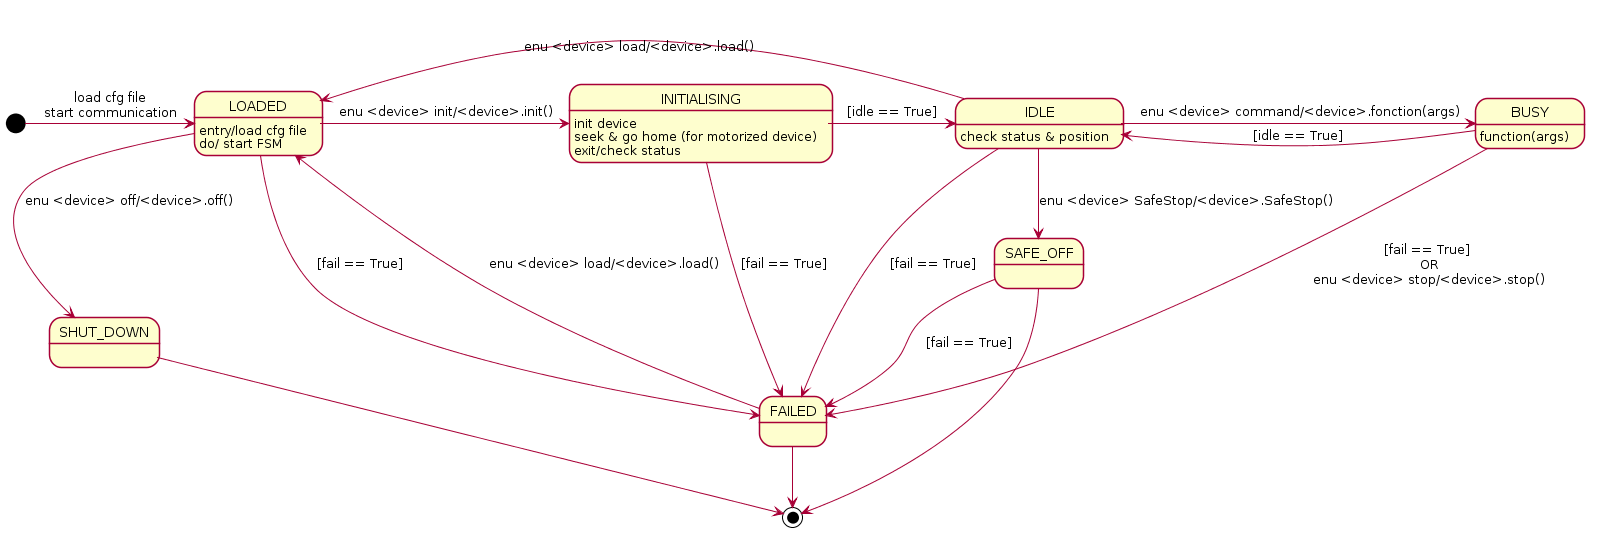
\includegraphics{../../state_diagram.png}\hfill}


\paragraph{The Devices}
\label{enuActor.Devices:the-devices}
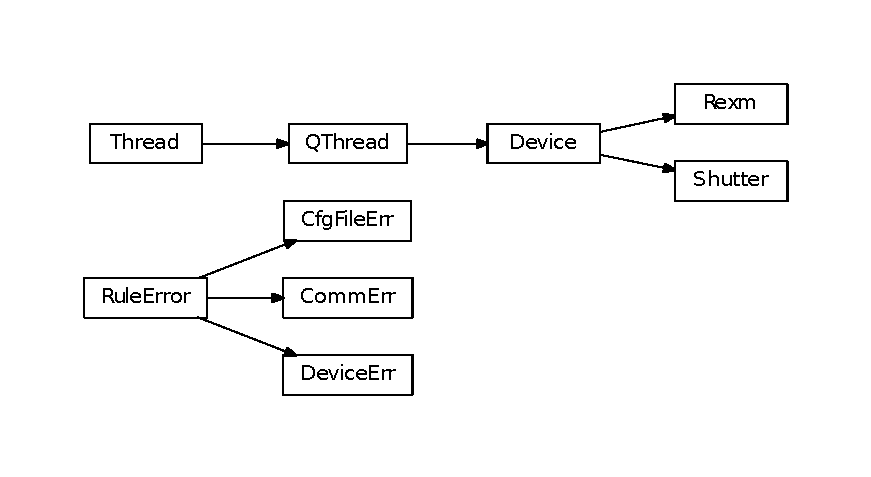
\includegraphics{inheritance-ffb85c930a227f83bc7b0e171aa07082f249b03a.pdf}


\subparagraph{Device}
\label{enuActor.Devices:device}
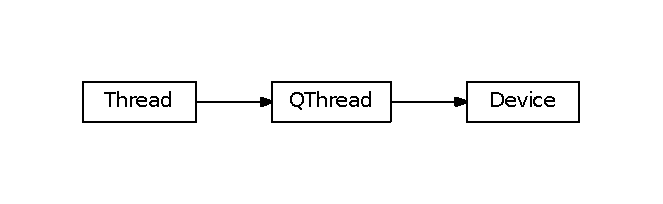
\includegraphics{inheritance-5ac211b25f8666d574d790775d7f5ea47d6b879b.pdf}


\subparagraph{Error}
\label{enuActor.Devices:error}
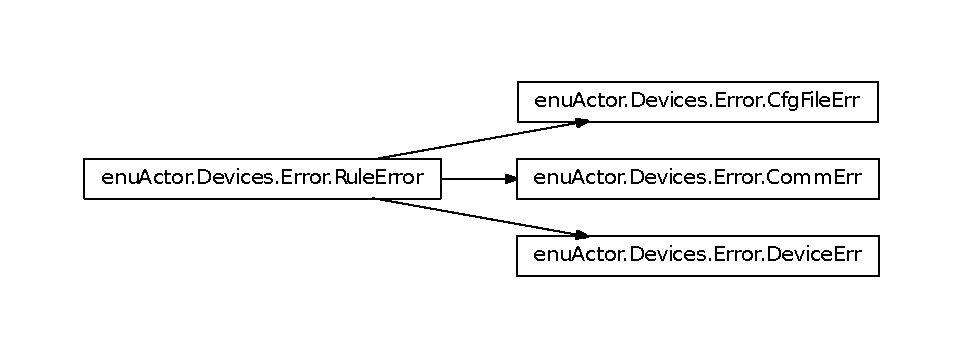
\includegraphics{inheritance-a934816c9f8b411a63067bc85b1ddf5dfcadc0b3.pdf}


\subparagraph{Shutter}
\label{enuActor.Devices:shutter}
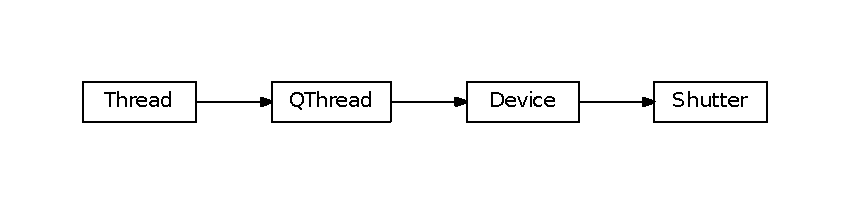
\includegraphics{inheritance-d3a48ebd57a6a6a4c1aee59224110dc9c5ab3113.pdf}

Shutter is open or close ...


\subparagraph{BIA}
\label{enuActor.Devices:bia}

\subparagraph{REXM}
\label{enuActor.Devices:rexm}
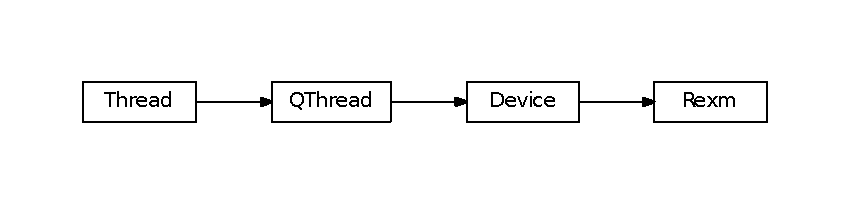
\includegraphics{inheritance-0a1a7ed4280ef7d9af164129c6e9afc50fd1ef14.pdf}


\subparagraph{IISOURCE}
\label{enuActor.Devices:iisource}

\subparagraph{ENU}
\label{enuActor.Devices:enu}

\subparagraph{FPSA}
\label{enuActor.Devices:fpsa}

\section{Submodules}
\label{enuActor:submodules}

\section{enuActor.DecoratorStateMachine module}
\label{enuActor:enuactor-decoratorstatemachine-module}\label{enuActor:module-enuActor.DecoratorStateMachine}\index{enuActor.DecoratorStateMachine (module)}\index{ContextBase (class in enuActor.DecoratorStateMachine)}

\begin{fulllineitems}
\phantomsection\label{enuActor:enuActor.DecoratorStateMachine.ContextBase}\pysigline{\strong{class }\code{enuActor.DecoratorStateMachine.}\bfcode{ContextBase}}
Bases: \code{object}

\end{fulllineitems}

\index{TransitionTable (class in enuActor.DecoratorStateMachine)}

\begin{fulllineitems}
\phantomsection\label{enuActor:enuActor.DecoratorStateMachine.TransitionTable}\pysiglinewithargsret{\strong{class }\code{enuActor.DecoratorStateMachine.}\bfcode{TransitionTable}}{\emph{stateVarblName}}{}
Bases: \code{object}

Defines a state table for a state machine class

A state table for a class is associated with the state variable in the instances
of the class. The name of the state variable is given in the constructor to the 
StateTable object.  StateTable objects are attributes of state machine classes, 
not intances of the state machine class.   A state machine class can have more
than one StateTable.
\index{initialize() (enuActor.DecoratorStateMachine.TransitionTable method)}

\begin{fulllineitems}
\phantomsection\label{enuActor:enuActor.DecoratorStateMachine.TransitionTable.initialize}\pysiglinewithargsret{\bfcode{initialize}}{\emph{ctxt}}{}
Create a new state variable in the context.  State variable refs this
transition table.

\end{fulllineitems}

\index{nextStates() (enuActor.DecoratorStateMachine.TransitionTable method)}

\begin{fulllineitems}
\phantomsection\label{enuActor:enuActor.DecoratorStateMachine.TransitionTable.nextStates}\pysiglinewithargsret{\bfcode{nextStates}}{\emph{subState}, \emph{nslList}}{}
Sets up transitions from the state specified by substate

subState is one of the derived state classes, subclassed from the
context state machine class. nslList is a list of states to which 
the context will transition upon the invocation of one of the 
transition methods.  `None' may be specified instead of an actual
state if the context is to remain in the same state upon invocation
of the corresponding method.

\end{fulllineitems}


\end{fulllineitems}

\index{event() (in module enuActor.DecoratorStateMachine)}

\begin{fulllineitems}
\phantomsection\label{enuActor:enuActor.DecoratorStateMachine.event}\pysiglinewithargsret{\code{enuActor.DecoratorStateMachine.}\bfcode{event}}{\emph{state\_table}}{}
Decorator for indicating an Event or `Action' method.

The decorator is applied to the methods of the state machine class to 
indicate that the method will invoke a state dependant behavior. States
are implemented as subclasses of the context(state machine) class .

\end{fulllineitems}

\index{transition() (in module enuActor.DecoratorStateMachine)}

\begin{fulllineitems}
\phantomsection\label{enuActor:enuActor.DecoratorStateMachine.transition}\pysiglinewithargsret{\code{enuActor.DecoratorStateMachine.}\bfcode{transition}}{\emph{state\_table}}{}
Decorator used to set up methods which cause transitions between states.

The decorator is applied to methods of the context (state machine) class. 
Invoking the method may cause a transition to another state.  To define
what the transitions are, the nextStates method of the TransitionTable class
is used.

\end{fulllineitems}

\index{transitionevent() (in module enuActor.DecoratorStateMachine)}

\begin{fulllineitems}
\phantomsection\label{enuActor:enuActor.DecoratorStateMachine.transitionevent}\pysiglinewithargsret{\code{enuActor.DecoratorStateMachine.}\bfcode{transitionevent}}{\emph{state\_table}}{}
A decorator which is essentially the combination of the above two.

Can both invoke state dependent method and trigger a state 
transition.  Mostly equivalent to :
@Transition(xitionTable)
@Event(xitionTable)

\end{fulllineitems}

\index{truncated() (in module enuActor.DecoratorStateMachine)}

\begin{fulllineitems}
\phantomsection\label{enuActor:enuActor.DecoratorStateMachine.truncated}\pysiglinewithargsret{\code{enuActor.DecoratorStateMachine.}\bfcode{truncated}}{\emph{alist}, \emph{cmprsn}}{}
\end{fulllineitems}



\section{enuActor.FSM module}
\label{enuActor:enuactor-fsm-module}

\section{enuActor.MyFSM module}
\label{enuActor:module-enuActor.MyFSM}\label{enuActor:enuactor-myfsm-module}\index{enuActor.MyFSM (module)}\index{Fysom (class in enuActor.MyFSM)}

\begin{fulllineitems}
\phantomsection\label{enuActor:enuActor.MyFSM.Fysom}\pysiglinewithargsret{\strong{class }\code{enuActor.MyFSM.}\bfcode{Fysom}}{\emph{cfg}}{}
Bases: \code{object}

Wraps the complete finite state machine operations.
\index{can() (enuActor.MyFSM.Fysom method)}

\begin{fulllineitems}
\phantomsection\label{enuActor:enuActor.MyFSM.Fysom.can}\pysiglinewithargsret{\bfcode{can}}{\emph{event}}{}
Returns if the given event be fired in the current machine state.

\end{fulllineitems}

\index{cannot() (enuActor.MyFSM.Fysom method)}

\begin{fulllineitems}
\phantomsection\label{enuActor:enuActor.MyFSM.Fysom.cannot}\pysiglinewithargsret{\bfcode{cannot}}{\emph{event}}{}
Returns if the given event cannot be fired in the current state.

\end{fulllineitems}

\index{is\_finished() (enuActor.MyFSM.Fysom method)}

\begin{fulllineitems}
\phantomsection\label{enuActor:enuActor.MyFSM.Fysom.is_finished}\pysiglinewithargsret{\bfcode{is\_finished}}{}{}
Returns if the state machine is in its final state.

\end{fulllineitems}

\index{isstate() (enuActor.MyFSM.Fysom method)}

\begin{fulllineitems}
\phantomsection\label{enuActor:enuActor.MyFSM.Fysom.isstate}\pysiglinewithargsret{\bfcode{isstate}}{\emph{state}}{}
Returns if the given state is the current state.

\end{fulllineitems}

\index{trigger() (enuActor.MyFSM.Fysom method)}

\begin{fulllineitems}
\phantomsection\label{enuActor:enuActor.MyFSM.Fysom.trigger}\pysiglinewithargsret{\bfcode{trigger}}{\emph{event}}{}
Triggers the given event.
The event can be triggered by calling the event handler directly, for ex: fsm.eat()
but this method will come in handy if the event is determined dynamically and you have
the event name to trigger as a string.

\end{fulllineitems}


\end{fulllineitems}

\index{FysomError}

\begin{fulllineitems}
\phantomsection\label{enuActor:enuActor.MyFSM.FysomError}\pysigline{\strong{exception }\code{enuActor.MyFSM.}\bfcode{FysomError}}
Bases: \code{exceptions.Exception}

Raised whenever an unexpected event gets triggered.

\end{fulllineitems}



\section{enuActor.QThread module}
\label{enuActor:module-enuActor.QThread}\label{enuActor:enuactor-qthread-module}\index{enuActor.QThread (module)}\index{QMsg (class in enuActor.QThread)}

\begin{fulllineitems}
\phantomsection\label{enuActor:enuActor.QThread.QMsg}\pysiglinewithargsret{\strong{class }\code{enuActor.QThread.}\bfcode{QMsg}}{\emph{method}, \emph{*argl}, \emph{**argd}}{}
Bases: \code{object}
\index{DEFAULT\_PRIORITY (enuActor.QThread.QMsg attribute)}

\begin{fulllineitems}
\phantomsection\label{enuActor:enuActor.QThread.QMsg.DEFAULT_PRIORITY}\pysigline{\bfcode{DEFAULT\_PRIORITY}\strong{ = 5}}
\end{fulllineitems}


\end{fulllineitems}

\index{QThread (class in enuActor.QThread)}

\begin{fulllineitems}
\phantomsection\label{enuActor:enuActor.QThread.QThread}\pysiglinewithargsret{\strong{class }\code{enuActor.QThread.}\bfcode{QThread}}{\emph{actor}, \emph{name}, \emph{timeout=2.0}, \emph{isDaemon=True}, \emph{queueClass=\textless{}class Queue.PriorityQueue at 0x341b0b8\textgreater{}}}{}
Bases: \code{threading.Thread}
\index{exitMsg() (enuActor.QThread.QThread method)}

\begin{fulllineitems}
\phantomsection\label{enuActor:enuActor.QThread.QThread.exitMsg}\pysiglinewithargsret{\bfcode{exitMsg}}{\emph{cmd=None}}{}
handler for the ``exit'' message. Spits out a message and arranges for the .run() method to exit.

\end{fulllineitems}

\index{handleTimeout() (enuActor.QThread.QThread method)}

\begin{fulllineitems}
\phantomsection\label{enuActor:enuActor.QThread.QThread.handleTimeout}\pysiglinewithargsret{\bfcode{handleTimeout}}{}{}
Called when the .get() times out. Intended to be overridden.

\end{fulllineitems}

\index{pingMsg() (enuActor.QThread.QThread method)}

\begin{fulllineitems}
\phantomsection\label{enuActor:enuActor.QThread.QThread.pingMsg}\pysiglinewithargsret{\bfcode{pingMsg}}{\emph{cmd=None}}{}
handler for the `ping' message.

\end{fulllineitems}

\index{putMsg() (enuActor.QThread.QThread method)}

\begin{fulllineitems}
\phantomsection\label{enuActor:enuActor.QThread.QThread.putMsg}\pysiglinewithargsret{\bfcode{putMsg}}{\emph{method}, \emph{*argl}, \emph{**argd}}{}
send ourself a new message.
\begin{quote}\begin{description}
\item[{Parameters}] \leavevmode\begin{itemize}
\item {} 
\textbf{method} -- a function or bound method to call

\item {} 
\textbf{*argl} -- the arguments to the method.

\item {} 
\textbf{*argd} -- the arguments dict to the method

\end{itemize}

\end{description}\end{quote}

\end{fulllineitems}

\index{run() (enuActor.QThread.QThread method)}

\begin{fulllineitems}
\phantomsection\label{enuActor:enuActor.QThread.QThread.run}\pysiglinewithargsret{\bfcode{run}}{}{}
Main run loop for this thread.

\end{fulllineitems}

\index{sendLater() (enuActor.QThread.QThread method)}

\begin{fulllineitems}
\phantomsection\label{enuActor:enuActor.QThread.QThread.sendLater}\pysiglinewithargsret{\bfcode{sendLater}}{\emph{msg}, \emph{deltaTime}, \emph{priority=1}}{}
Send ourself a QMsg after deltaTime seconds.

\end{fulllineitems}


\end{fulllineitems}



\section{enuActor.main module}
\label{enuActor:enuactor-main-module}

\section{Module contents}
\label{enuActor:module-enuActor}\label{enuActor:module-contents}\index{enuActor (module)}

\chapter{Indices and tables}
\label{index:indices-and-tables}\begin{itemize}
\item {} 
\emph{genindex}

\item {} 
\emph{modindex}

\item {} 
\emph{search}

\end{itemize}


\renewcommand{\indexname}{Python Module Index}
\begin{theindex}
\def\bigletter#1{{\Large\sffamily#1}\nopagebreak\vspace{1mm}}
\bigletter{e}
\item {\texttt{enuActor}}, \pageref{enuActor:module-enuActor}
\item {\texttt{enuActor.Commands}}, \pageref{enuActor.Commands:module-enuActor.Commands}
\item {\texttt{enuActor.DecoratorStateMachine}}, \pageref{enuActor:module-enuActor.DecoratorStateMachine}
\item {\texttt{enuActor.Devices}}, \pageref{enuActor.Devices:module-enuActor.Devices}
\item {\texttt{enuActor.Devices.Device}}, \pageref{enuActor.Devices:module-enuActor.Devices.Device}
\item {\texttt{enuActor.Devices.Error}}, \pageref{enuActor.Devices:module-enuActor.Devices.Error}
\item {\texttt{enuActor.Devices.rexm}}, \pageref{enuActor.Devices:module-enuActor.Devices.rexm}
\item {\texttt{enuActor.Devices.shutter}}, \pageref{enuActor.Devices:module-enuActor.Devices.shutter}
\item {\texttt{enuActor.MyFSM}}, \pageref{enuActor:module-enuActor.MyFSM}
\item {\texttt{enuActor.QThread}}, \pageref{enuActor:module-enuActor.QThread}
\end{theindex}

\renewcommand{\indexname}{Index}
\printindex
\end{document}
